\documentclass[11pt]{standalone}
\usepackage{amssymb}
\usepackage{amsmath}
\usepackage[no-math]{fontspec}
\usepackage{unicode-math}
\usepackage{libertinus}
\usepackage{pgf,xcolor}
\usepackage{tikz}
\usetikzlibrary{arrows.meta, backgrounds}
\usepackage{pgfplots}
\pgfplotsset{compat=newest}

\definecolor{my_darkgray}{HTML}{484949}
\definecolor{my_lightgray}{HTML}{F3F4F4}
\definecolor{my_darkblue}{HTML}{005A94}
\definecolor{my_lightblue}{HTML}{CCDEE9}
\definecolor{my_yellow}{HTML}{FFEC7F}
\definecolor{my_red}{HTML}{E60000}
\definecolor{my_orange}{HTML}{E87846}

\begin{document}
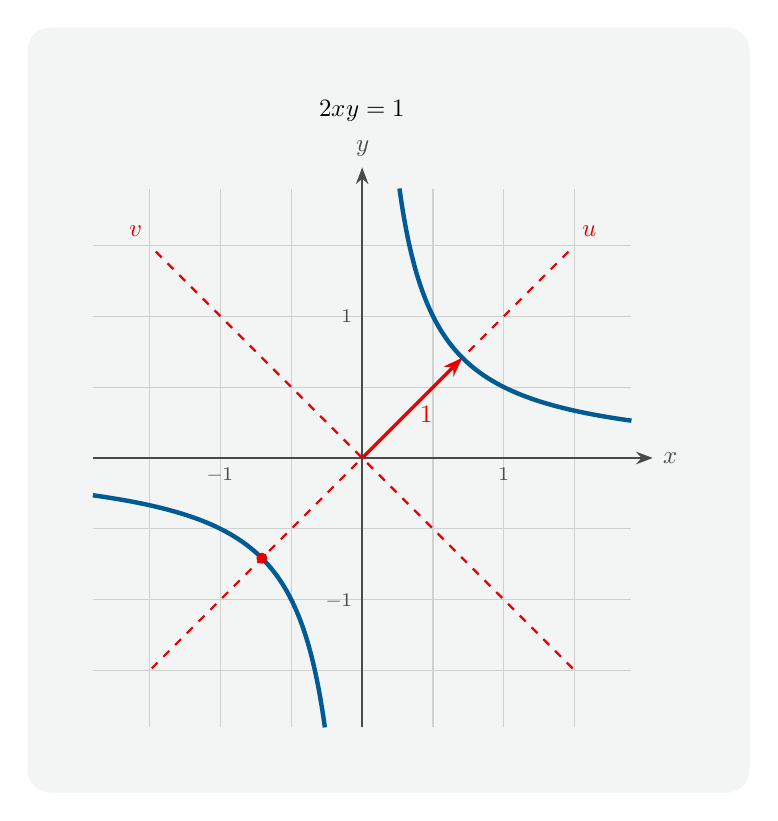
\begin{tikzpicture}[
    show background rectangle,
    background rectangle/.style={fill=my_lightgray, rounded corners=8pt},
    inner frame sep=0.8cm,
    x=1.8cm, y=1.8cm,
    vec/.style={-{Stealth[length=7pt, width=5pt]}, very thick}
]

% ---------------------------------------------------------------
%  2xy = 1, also y = 1/(2x), mit B = (0 1; 1 0)
%  Hauptachsen: u in Richtung (1, 1), v in Richtung (-1, 1), Q = R(45)
%  In Hauptachsen: u^2 - v^2 = 1, Scheitel bei u = +-1,
%  also bei x = +-(1, 1)/sqrt(2)
% ---------------------------------------------------------------

\draw[my_darkgray!25, thin, step=0.5] (-1.9, -1.9) grid (1.9, 1.9);

\begin{scope}[rotate=45]
    \draw[my_red, thick, dashed] (-2.1, 0) -- (2.1, 0)
        node[above right, font=\small, solid] {$u$};
    \draw[my_red, thick, dashed] (0, -2.1) -- (0, 2.1)
        node[above left, font=\small, solid] {$v$};
\end{scope}

\draw[-{Stealth[length=6pt]}, thick, my_darkgray] (-1.9, 0) -- (2.05, 0)
    node[right, font=\small] {$x$};
\draw[-{Stealth[length=6pt]}, thick, my_darkgray] (0, -1.9) -- (0, 2.05)
    node[above, font=\small] {$y$};
\foreach \t in {-1, 1}{
    \node[below, font=\scriptsize, my_darkgray] at (\t, 0) {$\t$};
    \node[left, font=\scriptsize, my_darkgray] at (0, \t) {$\t$};
}

\draw[my_darkblue, ultra thick] plot[domain=0.263:1.9, samples=150]
    (\x, {1/(2*\x)});
\draw[my_darkblue, ultra thick] plot[domain=-1.9:-0.263, samples=150]
    (\x, {1/(2*\x)});

\begin{scope}[rotate=45]
    \draw[vec, my_red] (0, 0) -- (1, 0);
    \node[below right, font=\small, my_red, inner sep=1pt] at (0.55, 0) {$1$};
    \fill[my_red] (-1, 0) circle[radius=2pt];
\end{scope}

\node[font=\small] at (0, 2.45) {$2xy = 1$};

\end{tikzpicture}
\end{document}
